\RequirePackage{tikz}
% Opcje klasy 'iithesis' opisane sa w komentarzach w pliku klasy. Za ich pomoca
% ustawia sie przede wszystkim jezyk i rodzaj (lic/inz/mgr) pracy, oraz czy na
% drugiej stronie pracy ma byc skladany wzor oswiadczenia o autorskim wykonaniu.
\documentclass[english,shortabstract,mgr]{iithesis}

\usepackage[utf8]{inputenc}
\usepackage{ulem}
\usepackage{amsthm}

%%%%% DANE DO STRONY TYTUŁOWEJ
% Niezaleznie od jezyka pracy wybranego w opcjach klasy, tytul i streszczenie
% pracy nalezy podac zarowno w jezyku polskim, jak i angielskim.
% Pamietaj o madrym (zgodnym z logicznym rozbiorem zdania oraz estetyka) recznym
% zlamaniu wierszy w temacie pracy, zwlaszcza tego w jezyku pracy. Uzyj do tego
% polecenia \fmlinebreak.
\polishtitle    {Tłumaczenie współczesnego języka programowania\fmlinebreak do Maszyny Minsky'ego.}
\englishtitle   {Modern programming language translation to the theoretical model of Minsky Machine (Counter Machine).}
\polishabstract {TODO: polishabstract}
\englishabstract{
Counter Machine (a machine with finite state set, two counters and input/output tape) is~able to express any
computations done by~modern programming languages. This is~the~well-known theorem, just like computations
performed using Turing Machine and~means that anything written in a~modern programming language is possible
to~translate into the~theoretical model of Minsky Machine (as well as into Turing Machine).

My goal is to build automatic translation from a~modern programming language (C++) to Minsky Machine.
}
% w pracach wielu autorow nazwiska mozna oddzielic poleceniem \and
\author         {Jadwiga Pokorska}
% w przypadku kilku promotorow, lub koniecznosci podania ich afiliacji, linie
% w ponizszym poleceniu mozna zlamac poleceniem \fmlinebreak
\advisor        {dr Jakub Michaliszyn}
%\date          {}                     % Data zlozenia pracy
% Dane do oswiadczenia o autorskim wykonaniu
\transcriptnum {247906}                     % Numer indeksu
\advisorgen    {dr Jakuba Michaliszyna} % Nazwisko promotora w dopelniaczu
%%%%%

%%%%% WLASNE DODATKOWE PAKIETY
%
%\usepackage{graphicx,listings,amsmath,amssymb,amsthm,amsfonts,tikz}
%
%%%%% WŁASNE DEFINICJE I POLECENIA
%
%\theoremstyle{definition} \newtheorem{definition}{Definition}[chapter]
%\theoremstyle{remark} \newtheorem{remark}[definition]{Observation}
%\theoremstyle{plain} \newtheorem{theorem}[definition]{Theorem}
%\theoremstyle{plain} \newtheorem{lemma}[definition]{Lemma}
%\renewcommand \qedsymbol {\ensuremath{\square}}
% ...
%%%%%

%\usepackage{todonotes}

\newcommand{\todo}[1]{\textbf{TODO:} #1}
\newtheorem*{hypothesis}{Hypothesis}

\begin{document}

%%%%% POCZĄTEK ZASADNICZEGO TEKSTU PRACY

\chapter{Introduction}

\section{Turing Machine}

Modern computers and their abilities nowadays are complex and depend on many different factors
to~perform given computations, like processor technology, software optimizations within given
processor model, input/output communication protocols and many others. This is why if we want
to~state or proof anything about the behaviour of computer programs then we need to~find a~common
language and~general theoretical model representing any type of "computer".

The model is known since 1936 when Alan Turing proposed something called \textbf{Turing Machine}
to represent a~machine that is able to~execute any computations expressible in~terms of~computer program.
It has all positive and~negative properties which belong to~modern programs, i.e. it~is possible
to create a~program which will never stop or~consume infinite amount of memory. The model does not allow
to~solve all the problems -- it~has got the~same limitations in~sense of~creating algorithms
like a~regular computer.

Turing Machine is~a~finite description of~an~algorithm and~uses potentially infinite tape
as~its memory -- we have some amount of~tape at~the beginning, but~we may extend this tape
(glue additional tape cells) to~the right end if necessary. All cells are either blank
or~contain a~single letter -- when machine starts its work there is an~input word
written on~the tape, during computations the~machine is allowed to~change all the available
cells and~after it finishes (if it finishes at all) it can either \textit{accept}
or~\textit{reject} original input word.

As~an~example we can try to construct Turing Machine recognizing all binary palindromes of~even length,
which is~formally set $A = \{ ww^R : w \in \{0,1\}^* \}$ (where $^R$ means reversing given word).

Because we need to use finite description to~define behaviour we say that the~machine should
check first letter $a_1$ with last one $a_n$ -- if these cells contain different letters machine
should reject the whole word, otherwise it should mark them as checked (i.e. write $\#$ symbol in~their cells)
and~continue with $a_2$ and~$a_{n-1}$. At~the~end we should have tape full of $\#$s and~the~machine
should accept given word. If there is just one unchanged cell left then it was a~palindrome
of~odd length and~we should reject it.

\textbf{Turing Machine} is a~$6$-tuple $(Q,\Sigma,\Gamma,\delta,q_0,P)$ where:
\begin{itemize}
  \item $Q$ is~a~finite set of~states the~machine can be within,
  \item $\Sigma$ is~a~finite input alphabet (does not contain blank),
  \item $\Gamma$ is~a~finite tape alphabet and~$\Sigma \subset \Gamma$,
  \item $\delta: Q \times \Gamma \rightarrow Q \times \Gamma \times \{L,R\}$ is~a~finite
      transition function, $L$ and~$R$ mean the~machine should move one cell left or~right
      respectively,
  \item $q_0$ is~the~initial state the~machine starts within,
  \item $P$ is~a~finite set of~states which accept input word.
\end{itemize}

\textbf{Configuration} of~a~Turing Machine consists of ($w$, $q$, $k$), where:
\begin{itemize}
  \item $w \in \Sigma^*$ is a~word initially written on~the~tape,
  \item $q$ is a~state of the~machine is~currently within,
  \item $k$ is a~cell number the~machine is currently looking at.
\end{itemize}

Having a~configuration we can precisely say what is the~program execution progress.
One configuration is~a~precise step of~computation, so a~sequence of~configurations is called
a~\textbf{run} of~a~Turing Machine. This sequence may be finite or~infinite the~same way like
a~program may loop forever or~finish within some number of~steps. Each such run begins with
a~configuration where some word $w$ is~an~input, $k = 0$ which is the~leftmost cell on~the~tape
and~$q = q_0$ which is initial state defined in~the~description of~given machine. If~a~run is
finite and~ends with configuration ($w_n$, $q_n$, $k_n$) then we define the~input word to~be
\textit{accepted} if $q_n \in P$ ($q_n$ is one of accepting states) and \textit{rejected} otherwise.

\section{Church-Turing thesis and Turing-completeness}

Computers are used to perform calculations for us, more precicely we want them to~execute some
procedures or~to~perform some process and~we call it an~\textit{algorithm} in~its intuitive meaning.
A~good example could be~a~mathematical problem of~generating prime numbers -- it~is fairly simple
to~think of~a~method of~generating prime numbers by checking lager and~larger numbers and~checking
their all possible divisors. We~are able to~precisely say what this algorithm looks like and~if
we think for a~while we would probably be able to~express it in terms of Turing Machines. That
is~exactly what \textbf{Church-Turing thesis} states:

\begin{hypothesis}
  Intuitive definition of~any~algorithm is~equivalent to~some description of~Turing Machine.
\end{hypothesis}

This thesis allows us to~think about defining algorithms in~intuitive way while still staying
within the~world of~Turing Machine programs.

It~turns out that when designing any~modern algorithms we use~the same way of~intuitive description
of~a~procedure and~then we~are converting it~into \textit{implementation} which is~a~representation
of~given algorithm using a~modern programming language. From thesis above we~claim that most probably
it~would be~possible to~express it~as~a~Turing Machine (but probably require lots of~thought).

To~avoid~a~painful process of~expressing algorithms in~an~unhandy theoretical model we~have
a~concept of~\textbf{Turing-completeness}. All popular modern programming languages are proven
to~be Turing-complete which means that we are able to~implement our algorithm in~such
language if and only if there exists some equivalent Turing Machine description.

\section{Counter Machine}

We have so far theoretical model -- Turing Machine -- which has the~same power of~expression
as~modern languages and~it turns out there are many others we~can describe and~prove they are
equivalent to Turing Machine (so~to~modern languages as~well). One of~such alternatives
is~\textbf{Counter Machine} (sometimes called \textbf{Minsky Machine}) which is~really primitive
in~its construction.

Similarly to~Turing Machine, Counter Machine has~finite description -- finite set of~states $Q$
and~transition function $\delta$ defining when the~machine may move from one state to~another.
Instead of~the~infinite tape there are $2$ counters -- each counter works like a~glass of~coins,
the~machine may throw a~coin (or~several coins) into the~glass, check whether the~glass is~empty
or~take out a~coin (only one and~only if glass is not empty). Each counter is~basically a~non-negative
integer, but the~machine is~not allowed to~explicitly check its value, it~just gets boolean
information about emptiness.

There are a~few alternative models -- if~we~allow the~machine to~use $3$ counters instead of~$2$
then we get equivalent model, the~same for $4$ or~more counters. According to~this fact, we~can
choose how many counters it~is convenient for~us to~use. The~only exception is~Counter Machine with
$1$ counter which is~not able to~express everything a~$2$ Counter Machine can -- TODO: jaką klasę
języków możemy wyrazić?

\section{Brainfuck}

As~we defined above Counter Machine is~a~minimalistic model of~computations, the~same way
\textbf{Brainfuck} is a~minimalistic programming language which recalls the~definition
of~Turing Machine -- program operates on~a~tape containing numbers, it~is possible
to~explicitly read and~change values in~cells. A~program operates on~a~data pointer which
points to~the~current focus cell, so~that it~is able to~freely move around. The~main difference
between Turing Machine and~Brainfuck is~lack of~states and~transitions, instead a~program
is a~sequence of intructions that are executed one by~one.

Usually Brainfuck implementations assume that tape length is~around $30\,000$ cells which
is~enough in~most cases. If~we want to~prove Turing-completeness though, this tape
needs to~be potentially infinite. Of couse, no~modern machine is~equipped with infinite memory,
but we are able to~extend it (with buying additional hardware), so~this factor is~omitted
when proving Turing-completeness. It is not a~problem in~this thesis at~all since
the~main goal is to~show that anything written in~modern programming language is~possible
to~automatically translate into~theoretical model.

\section {Purpose of this thesis}

This~thesis should be~a~proof of~theoretical concept contained in~Church-Turing thesis -- any~algorithm
or~mathematical method we~are able to~come up with (as~long as it is expressible in any programming
language) is possible to~execute on~the~most primitive theoretical model which is~Counter Machine.

Implementation translates Brainfuck into Counter Machine model and~consists of~a~few separate parts
which are completely separate translations between more and more primitive theoretical models.
It is possible to access any transitional (temporary) programs created during the~whole process.

The~plan for translation that shows what is~generated as~transitional models:

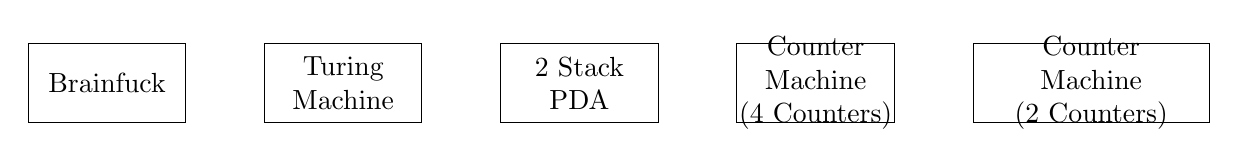
\begin{tikzpicture}
  \draw (0,0) rectangle (2,1) node[pos=.5] {Brainfuck};
  \draw (3,0) rectangle (5,1) node[pos=.5, text width=2cm, align=center] {Turing Machine};
  \draw (6,0) rectangle (8,1) node[pos=.5, text width=2cm, align=center] {2 Stack PDA};
  \draw (9,0) rectangle (11,1) node[pos=.5, text width=2.5cm, align=center] {Counter Machine \\ (4 Counters)};
  \draw (12,0) rectangle (15,1) node[pos=.5, text width=2.5cm, align=center] {Counter Machine \\ (2 Counters)};
\end{tikzpicture}

\todo{Co to są \sout{maszyny Turinga, Mińskiego, Brainfuck, Turning-zupełność, hipoteza Churcha}}

\todo{O czym jest ta praca - lista kontrybucji}

\todo{\sout{Po co jest ta praca --- ,,proof of concept''; ,,walory dydaktyczne'', }\dots}

\todo{,,Related work''}

\todo{Plan pracy}

\ldots

\chapter {Preliminaries}

\section {Brainfuck}

Brainfuck is a programming language with only $8$ statements and execution
of~any program is done using a~finite sequence of~memory cells. Statements
operate on~these cells using data pointer --- initially the pointer is set
on the~leftmost cell in the sequence.

Statements:
\begin{itemize}
  \item \texttt{>} moves the data pointer one cell to the right,
  \item \texttt{<} moves the data pointer one cell to the left,
  \item \texttt{+} increase by $1$ the value held in the cell under the data pointer,
  \item \texttt{-} decrease by $1$ the value held in the cell under the data pointer,
  \item \texttt{.} print to stdout the~character that is under the~data pointer,
  \item \texttt{,} read from stdin a~character and write it to the cell under the data pointer,
  \item \texttt{$[$} beginning of a loop with condition checking whether value under
      the~data pointer is zero. If it is then execution jumps to the matching $]$,
  \item \texttt{$]$} closing symbol of a loop --- execution jumps to the~beginning of the~loop
      (matching $[$) and then check for zero value under the data pointer is performed.
\end{itemize}

It is allowed to use any other characters within the code, but anything else than the $8$
listed above are ignored --- it is useful for creating comments in the code.

An example code printing "Hello World!":
\begin{verbatim}
++++++++++
[
>+++++++>++++++++++>+++>+<<<<-
] We set up the values in few cells for future use.
>++.               prints 'H'
>+.                prints 'e'
+++++++.           prints 'l'
.                  prints 'l'
+++.               prints 'o'
>++.               prints space
<<+++++++++++++++. prints 'W'
>.                 prints 'o'
+++.               prints 'r'
------.            prints 'l'
--------.          prints 'd'
>+.                prints '!'
>.                 prints newline character
\end{verbatim}

\section {Turing Machine}

\subsection {Instructions}

Turing Machine consists of a finite number of states, changes between them
and~potentially infinite tape, on~which it is able to~write and~read symbols.
It has no code sequence, a program is a~set of state changes and~definition
of~an~initial state. There is special final state \texttt{END} that does not need
        to~be defined to~be used.

There is a~predefined set of symbols used on the tape which is whole ASCII character set
extended with the same amount of additional (non-ASCII) symbols. Regular
ASCII characters have 7 bits (numbers 0-127), so tape symbols have 8 bits
allowing to hold regular ASCII and special characters (numbers 128-255).

        There are few special definitions (so far using regular ASCII,
but it will be changed to use special characters instead):
\begin{itemize}
  \item \texttt{BLANK} which represents empty field on the tape
  \item \texttt{*} (ALL) defines all characters (both ASCII and special)
  \item \texttt{\#} (NOTHING) means no character which is used to say
                   that we do not want to write anything on tape during
                   this state change
          \item \texttt{\&} (NON-ZERO) defines all characters except 0
          \item \texttt{0} (ZERO) represents zero that is used for conditional jumps
           (jump zero)
          \item \texttt{>} (NEXT-CHAR) allows writing on the tape next character
                   (increased by one), i.e. writes \texttt{g} if on the tape
                   was \texttt{f}
  \item \texttt{<} (PREV-CHAR) similarly as above but writes the previous character,
                   i.e. writes \texttt{e} when seen \texttt{f}
\end{itemize}

Defining initial state:
\begin{verbatim}
START: state_name
\end{verbatim}

Each state change looks as follows:
\begin{verbatim}
state_name symbol(s) -> target_state head_move symbol_to_write
\end{verbatim}

\texttt{symbol(s)} is ASCII character including special definitions (currently
all special definitions use regular ASCII so that it is easy to see
in a~standard text file), in future it will allow getting non-ASCII special
characters as well.

\texttt{head move} is one of \texttt{L}, \texttt{R} or \texttt{-} which
steer the head to go left, right or stay in place, respectively.

\texttt{symbol to write} is any (currently ASCII) symbol. Currently, there
is no mechanism to prevent writing any symbol from special definitions,
but~it will cause an~undefined behaviour of~the machine. The only symbol
from special definitions that is allowed to appear as \texttt{symbol\_to\_write}
is \texttt{\#} (NOTHING) meaning that symbol on the tape should not change.

\subsection {Extensions of the theoretical model}

Standard input/output handling is done by allowing to read or write single
ASCII character from/to stdin/stdout. It is possible to~add additional
reading or~writing before moving the~head. It is done by modifying change
symbol \texttt{->} in the~state change definition.
\begin{itemize}
  \item Reading is done with \texttt{->*}, i.e. \texttt{state1 A ->* state2 R NOTHING}
        which means when seen symbol \texttt{A} in state \texttt{state1} we read
        from stdin one character, overwrite \texttt{A} to read value and move
        head one field right.
  \item Writing is done similarly with \texttt{->\^},
        i.e. \texttt{state1 A ->\^ state2 R NOTHING} which will print symbol
        \texttt{A} on stdout and move the~head to the~right.
\end{itemize}

\subsection{Example}

A~program that reads a~letter from stdin, writes this letter into
stdout and if the~written letter was \texttt{B} or \texttt{b} then prints
\texttt{.} at the end as well, otherwise finishes.

\begin{verbatim}
START: s1
s1 ALL ->* s2 - NOTHING
s2 ALL ->^ s3 - NEXT_CHAR
s3 ALL -> s4 - NOTHING
s4 b ->^ s5 R NOTHING
s4 B ->^ s5 R NOTHING
s5 ALL -> s6 - .
s6 ALL ->^ s7 - NOTHING
s7 ALL -> END - NOTHING
\end{verbatim}

Note: If there is no state change defined for given configuration
(nothing matches) then it is assumed that machine gets to \texttt{END} state.
Because of this in the above example, last instruction is not necessary.

\section {2 Stack Pushdown Automaton}

2 Stack Pushdown Automaton consists of two stacks, input tape and~definition
of~states and transitions between them. Each transition looks as follows:
\begin{verbatim}
state_name left_pattern right_pattern ->
    target_state left_stack_items right_stack_items
\end{verbatim}

Explanation:
\begin{itemize}
  \item \texttt{left\_pattern} is symbol or pattern that should be matched
      for the symbol at the top of the left stack
  \item \texttt{right\_pattern} is the same as above, but for right stack
  \item \texttt{left\_stack\_items} are the list of items that should be pushed
      to the~left stack before moving to \texttt{target\_state}. It might be
      a~single letter \texttt{"a"}, a~sequence of letters \texttt{"abc"}
      or~sequence of~letters and~references, i.e. \texttt{("a" + ORIG\_LEFT + "b")}
      where \texttt{ORIG\_LEFT} means the letter we read from the~left stack (the one matched
      in \texttt{left\_pattern}). Note: If \texttt{+} is used it is required to put
      the~whole sequence in parenthesis
  \item \texttt{right\_stack\_items} are the same as above, but for items to be pushed into right stack
\end{itemize}

Special references and definitions in transitions:
\begin{itemize}
  \item \texttt{ORIG\_LEFT} is the letter taken from the left stack
  \item \texttt{ORIG\_RIGHT} is the letter taken from right stack
  \item \texttt{INPUT\_CHAR} is the letter taken from input tape
      (only in input transition type - see section below)
  \item \texttt{NOTHING} may be used as \texttt{left\_stack\_items} or \texttt{right\_stack\_items}
      and means that nothing is pushed into left/right stack
  \item \texttt{END} is special state name into which the transition is made if no other transition is specified
  \item \texttt{\$} is the symbol of the empty stack
\end{itemize}

\subsection {Extensions of the theoretical model}

Input/Output handling is done similarly to Turing Machine - We change \texttt{->} in transition
to \texttt{->*} or \texttt{->\^}.

When defining input transition it is allowed to use \texttt{INPUT\_CHAR} in any items
to be pushed into left/right stack. Here is an~example that takes a~character from input
tape and pushes it into the~left stack (and ignores symbols taken from both stacks).
\begin{verbatim}
state1 ALL ALL ->* state2 INPUT_CHAR NOTHING
\end{verbatim}

When defining output transition we \textbf{must} specify what character is printed
with adding \texttt{Output: <letter>} at the very back of transition definition.
An~example that prints letter taken from the~left stack (and ignores what was taken from right stack):
\begin{verbatim}
state1 ALL ALL ->^ state2 NOTHING NOTHING Output: ORIG_LEFT
\end{verbatim}
An~example that prints letter "a" (and ignores what was taken from stacks):
\begin{verbatim}
state1 ALL ALL ->^ state2 NOTHING NOTHING Output: "a"
\end{verbatim}

\textbf{Important note:} Order of defining transition matters. If patterns do not match
a~distinct set of letters then the transition that appeared first is applied.

\subsection{Example}

An~example (equivalent to the example from Turing Machine):
\begin{verbatim}
START: init_state
init_state $ $ -> s1 BLANK NOTHING
s1 ALL ALL ->* s2 INPUT_CHAR ORIG_RIGHT
s2 ALL ALL ->^ s3 ORIG_LEFT ORIG_RIGHT Output: ORIG_LEFT
s3 b $ -> s4 (ORIG_LEFT + BLANK) $
s3 b ALL -> s4 (ORIG_LEFT + ORIG_RIGHT) NOTHING
s3 B $ -> s4 (ORIG_LEFT + BLANK) $
s3 B ALL -> s4 (ORIG_LEFT + ORIG_RIGHT) NOTHING
s4 ALL ALL -> s5 "." ORIG_RIGHT
s5 ALL ALL ->^ s6 ORIG_LEFT ORIG_RIGHT Output: ORIG_LEFT
s6 ALL ALL -> END ORIG_LEFT ORIG_RIGHT
\end{verbatim}

\section {Counter Machine (4 counters)}

Counter Machine consists of $4$ counters each holding non-negative integer,
a~finite number of states and~transitions between them. Each transition
looks as follows:

\begin{verbatim}
state_name (pattern pattern pattern pattern) ->
    target_state (number number number number)
\end{verbatim}

Where:
\begin{itemize}
  \item \texttt{state\_name} is the state in which counter machine needs to be
      within for this transition to be applied,
  \item \texttt{pattern} is one of values \texttt{0}, \texttt{1} or \texttt{\_}
      meaning empty counter, non-empty counter and any counter state and defines
      what is expected state of the~given counter - the transition may be applied
      only when all counter states are matched (Notice that symbol \texttt{\_}
      is matched with any state of the counter),
  \item \texttt{target state} is the state in which machine will be after
      applying the transition,
  \item \texttt{number} is an~integer from the~range \texttt{[-1, MAX\_INT]} specifying
      what should be added to given counter - it is allowed to decrease counter
      by $1$ only, but it is possible to increase it by any number that can be stored
      in regular integer type.
\end{itemize}

\textbf{Note:} If there are many transitions that may be applied in given state
matching all counters \textbf{the first one} is applied. It means that order
of defining transitions matters.

It is required to give an~initial state of the machine with the following statement:
\begin{verbatim}
START: state_name
\end{verbatim}

\subsection {Extensions of the theoretical model}

Input/Output operations fit in the schema of using counters - input and output
are additional counters which transitions may use in a~similar way as counters are used.

Input transition is defined as follows:
\begin{verbatim}
state_name (counters) input pattern ->*
    target_state (numbers) input_operation
\end{verbatim}

Where:
\begin{itemize}
  \item \texttt{input\_pattern} is one of \texttt{0}, \texttt{1} or \texttt{\_}
      (same as counter pattern) and specifies what should be the state
      of input counter for this transition to be applied,
  \item \texttt{input\_operation} specifies what action should be performed
      on input counter and is one of \texttt{LOAD}, \texttt{-1} or \texttt{NOOP}
      meaning respectively loading a~character from stdin into the input counter,
      decrease input counter by \texttt{1} and leaving input counter untouched.
\end{itemize}

This transition reads from stdin into input counter:
\begin{verbatim}
state1 (_ _ _ _) _ ->* state2 (0 0 0 0) LOAD
\end{verbatim}

These transitions read the~value from input counter and store it in first counter:
\begin{verbatim}
state1 (_ _ _ _) 1 ->* state1 (1 0 0 0) -1
state1 (_ _ _ _) 0 ->* state2 (0 0 0 0) NOOP
\end{verbatim}

Note: It is assumed that transition may just decrease the input counter
and is not allowed to increase its value directly.

Output transition is defined as follows:
\begin{verbatim}
state_name (counters) ->^ target_state (numbers) Output: output_operation
\end{verbatim}

Where:
\begin{itemize}
  \item \texttt{output\_operation} specifies what should be performed
      on output counter and may be one of \texttt{FLUSH} or non-negative number,
      meaning respectively pushing counter to stdout and modifying
      the~value stored in the counter by the~given number.
\end{itemize}

These transitions print character stored in first counter:
\begin{verbatim}
state1 (1 _ _ _) ->^ state1 (-1 0 0 0) Output: 1
state1 (0 _ _ _) ->^ state2 (0 0 0 0) Output: FLUSH
\end{verbatim}

Note: It is assumed that transition may just increase the output counter
and is not allowed to decrease its value directly.


\subsection{Example}

Code that reads a~character from stdin doubles its ASCII value and prints the result.
\begin{verbatim}
START: s1
s1 (_ _ _ _) _ ->* s2 (0 0 0 0) LOAD
s2 (_ _ _ _) 1 ->* s2 (1 0 0 0) -1
s2 (_ _ _ _) 0 ->* s3 (0 0 0 0) NOOP
s3 (1 _ _ _) -> s3 (-1 2 0 0)
s3 (0 _ _ _) -> s4 (0 0 0 0)
s4 (_ 1 _ _) ->^ s4 (0 -1 0 0) Output: 1
s4 (_ 0 _ _) ->^ END (0 0 0 0) Output: FLUSH
\end{verbatim}

\section {Counter Machine (2 counters)}

Counter Machine with 2 counters has the same definition as
Counter Machine with 4 counters, but it is allowed to use only
2 counters, so transitions become of the form:

\begin{verbatim}
state_name (pattern pattern) -> target_state (number number)
\end{verbatim}

Input/Output is handled the same way it is handled in Counter Machine with 4 counters.


\chapter{Theoretical underpinnings}

\todo{O tym, jak te redukcje działają}

\chapter{Implementation}

\section{Ogólny wstęp}

\todo{Uzasadnienie doboru narzędzi}

\todo{Najciekawsze wyzwania}

\todo{Wszystko, co było ciekawe}

\section{Szczegóły techniczne}

\todo{Co jest gdzie, jak to się uruchamia, itd. / skrócona instrukcja użytkownika}

\todo{Ograniczenia implementacji}

\section{Przykłady}

Dużo przykładów...

\section{Ewaluacja}

Porównanie czasów

Tabelka

\section{Optymalizacje}

\chapter{Podsumowanie, wnioski, możliwości kontynuowania}

\appendix

\chapter{Szczegółowy sposób instalacji i konfiguracji lub dostępu do działającego systemu oraz podręcznik użytkownika systemu.}

%%%%% BIBLIOGRAFIA

%\begin{thebibliography}{1}
%\bibitem{example} \ldots
%\end{thebibliography}

\end{document}
